
\begin{center}
	\tcbox[colback=magenta!25!white,colframe=magenta, title=Teorema]{Los motores eléctricos son máquinas que transforman la energía eléctrica en movimiento (energía cinética). Estos aparatos se componen, básicamente, del rotor y de un estator donde tiene bobinas inductoras desfasadas entre sí 120°.}
\end{center}
		
	

\subsubsection{Especificaciones}

	El motor (Figura \ref{fig:motor}) asincrónico que se utiliza es de la marca \textbf{Altium} perteneciente a la firma \textbf{Schneider Electric}. Las especificaciones se muestran a continuación \\
	\paragraph*{Altium Eff2}
	\begin{itemize}
		\item 	Tipo: TE2A90SP2
		\item   Tensión nominal: 220/380 V
		\item 	Corriente nominal: 5.97 A 
		\item	Frecuencia nominal:  50 Hz.
		\item 	Potencia: 1.5kW / 2 HP
		\item 	Fases: 3
		\item   Factor de Potencia: 0.84
	\end{itemize}
	\newpage
	\begin{figure}[h!]
		\centering
		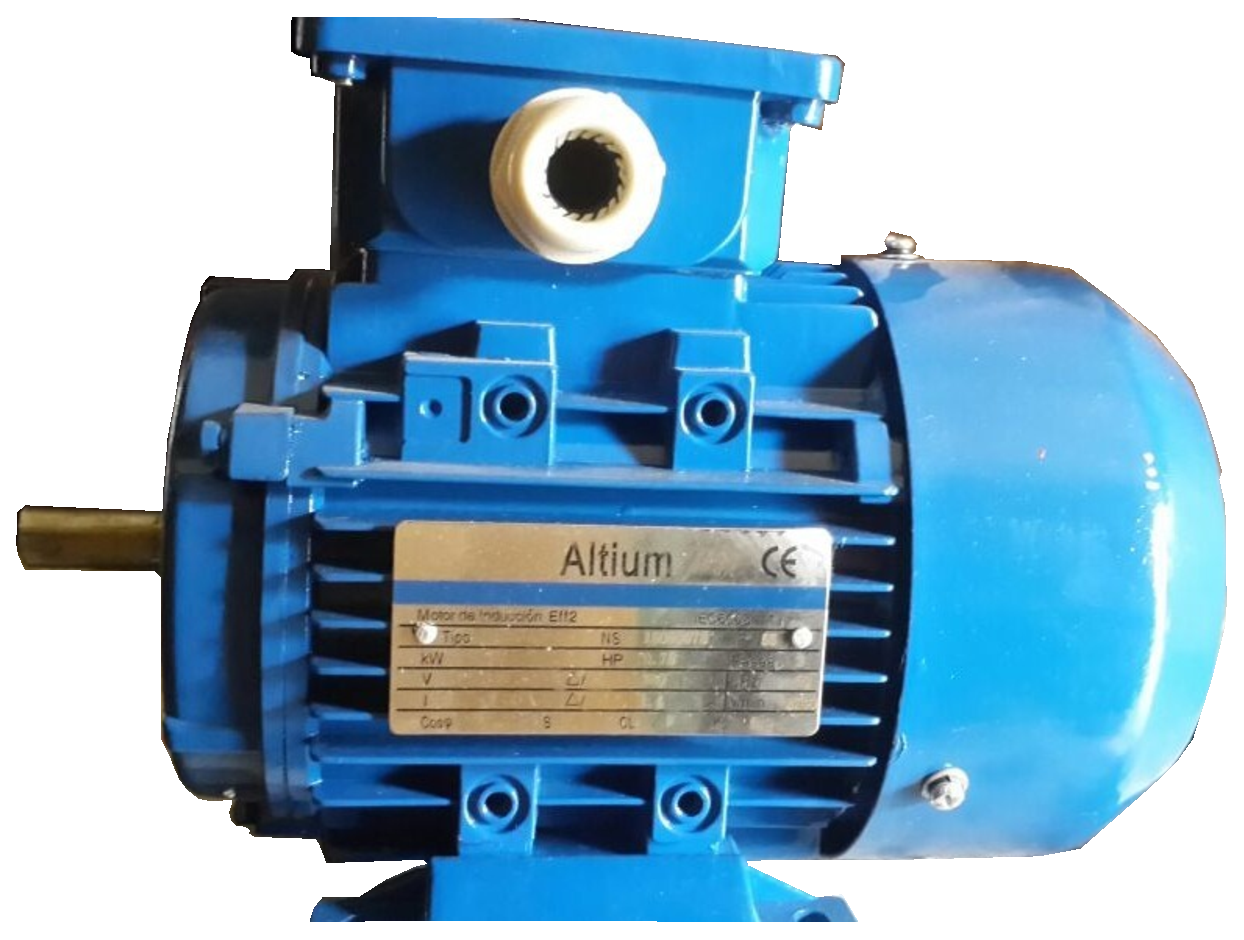
\includegraphics[scale=0.4]{motor.eps}
		\caption{Motor Altium}
		\label{fig:motor}
	\end{figure}
	\newpage